\documentclass{standalone}
\usepackage{tikz}
\usetikzlibrary{patterns, positioning}
\usepackage[sfdefault]{ClearSans} %% option 'sfdefault' activates Clear Sans as the default text font
\usepackage[T1]{fontenc}

\begin{document}
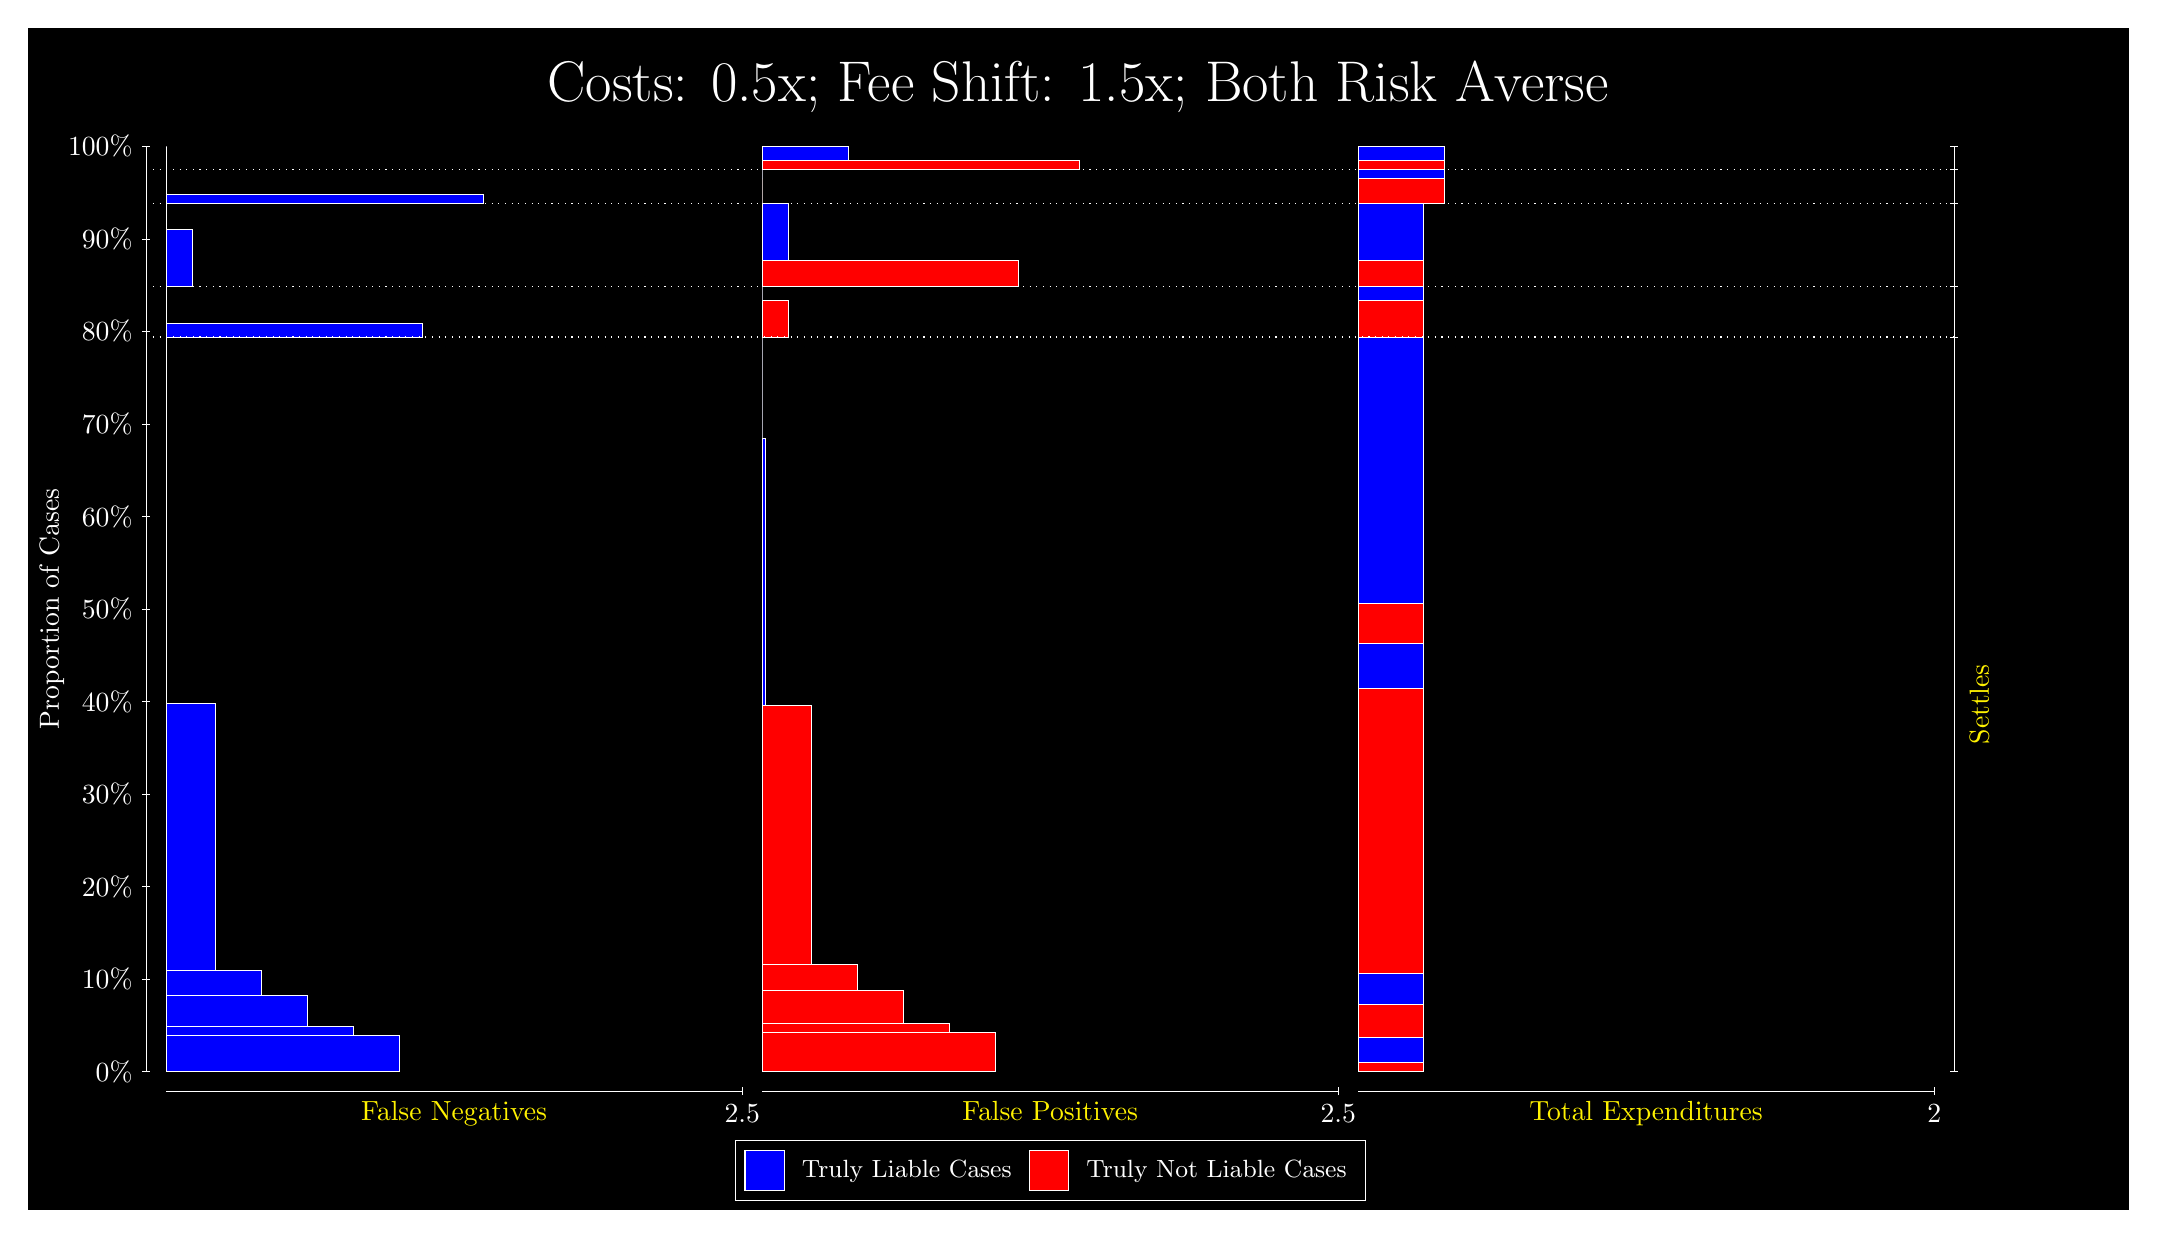
\begin{tikzpicture}
\draw[fill=black] (0,0) rectangle (26.667,15);
\draw[text=white] (0,13.5) rectangle (26.667,15) node[midway] {\huge Costs: 0.5x; Fee Shift: 1.5x; Both Risk Averse};
\draw[white, very thin] (1.5,1.75) -- (1.5,13.5);
\node[rotate=90, text=white, anchor=center] at (0.3, 7.625) {Proportion of Cases};
\draw[white, very thin] (1.45,1.75) -- (1.55,1.75);
\node[text=white, anchor=east] at (1.45, 1.75) {0\%};
\draw[white, very thin] (1.45,2.925) -- (1.55,2.925);
\node[text=white, anchor=east] at (1.45, 2.925) {10\%};
\draw[white, very thin] (1.45,4.1) -- (1.55,4.1);
\node[text=white, anchor=east] at (1.45, 4.1) {20\%};
\draw[white, very thin] (1.45,5.275) -- (1.55,5.275);
\node[text=white, anchor=east] at (1.45, 5.275) {30\%};
\draw[white, very thin] (1.45,6.45) -- (1.55,6.45);
\node[text=white, anchor=east] at (1.45, 6.45) {40\%};
\draw[white, very thin] (1.45,7.625) -- (1.55,7.625);
\node[text=white, anchor=east] at (1.45, 7.625) {50\%};
\draw[white, very thin] (1.45,8.8) -- (1.55,8.8);
\node[text=white, anchor=east] at (1.45, 8.8) {60\%};
\draw[white, very thin] (1.45,9.975) -- (1.55,9.975);
\node[text=white, anchor=east] at (1.45, 9.975) {70\%};
\draw[white, very thin] (1.45,11.15) -- (1.55,11.15);
\node[text=white, anchor=east] at (1.45, 11.15) {80\%};
\draw[white, very thin] (1.45,12.325) -- (1.55,12.325);
\node[text=white, anchor=east] at (1.45, 12.325) {90\%};
\draw[white, very thin] (1.45,13.5) -- (1.55,13.5);
\node[text=white, anchor=east] at (1.45, 13.5) {100\%};

\draw[white, very thin] (24.457,1.75) -- (24.457,13.5);
\draw[white, very thin] (24.407,1.75) -- (24.507,1.75);
\node[anchor=west] at (24.407, 1.75) {};
\draw[white, very thin] (24.407,11.078) -- (24.507,11.078);
\node[anchor=west] at (24.407, 11.078) {};
\draw[white, very thin] (24.407,11.719) -- (24.507,11.719);
\node[anchor=west] at (24.407, 11.719) {};
\draw[white, very thin] (24.407,12.775) -- (24.507,12.775);
\node[anchor=west] at (24.407, 12.775) {};
\draw[white, very thin] (24.407,13.206) -- (24.507,13.206);
\node[anchor=west] at (24.407, 13.206) {};
\draw[white, very thin] (24.407,13.5) -- (24.507,13.5);
\node[anchor=west] at (24.407, 13.5) {};

\draw[white, very thin, fill=blue] (1.75,1.75) rectangle (4.7141,2.2087);
\draw[white, very thin, fill=blue] (1.75,2.2087) rectangle (4.1286,2.3223);
\draw[white, very thin, fill=blue] (1.75,2.3223) rectangle (3.5431,2.715);
\draw[white, very thin, fill=blue] (1.75,2.715) rectangle (2.9576,3.0389);
\draw[white, very thin, fill=blue] (1.75,3.0389) rectangle (2.3721,6.4262);
\draw[white, very thin, fill=red] (1.75,6.4262) rectangle (1.75,11.078);
\draw[white, very thin, fill=blue] (1.75,11.078) rectangle (5.0069,11.257);
\draw[white, very thin, fill=red] (1.75,11.257) rectangle (1.75,11.719);
\draw[white, very thin, fill=blue] (1.75,11.719) rectangle (2.0793,12.445);
\draw[white, very thin, fill=red] (1.75,12.445) rectangle (1.75,12.775);
\draw[white, very thin, fill=blue] (1.75,12.775) rectangle (5.7754,12.894);
\draw[white, very thin, fill=red] (1.75,12.894) rectangle (1.75,13.206);
\draw[white, very thin, fill=red] (1.75,13.206) rectangle (1.75,13.325);
\draw[white, very thin, fill=blue] (1.75,13.325) rectangle (1.75,13.5);
\draw[white, very thin, fill=red] (9.3189,1.75) rectangle (12.283,2.2533);
\draw[white, very thin, fill=red] (9.3189,2.2533) rectangle (11.697,2.3669);
\draw[white, very thin, fill=red] (9.3189,2.3669) rectangle (11.112,2.7839);
\draw[white, very thin, fill=red] (9.3189,2.7839) rectangle (10.526,3.1078);
\draw[white, very thin, fill=red] (9.3189,3.1078) rectangle (9.941,6.4021);
\draw[white, very thin, fill=blue] (9.3189,6.4021) rectangle (9.3555,9.7894);
\draw[white, very thin, fill=blue] (9.3189,9.7894) rectangle (9.3189,11.078);
\draw[white, very thin, fill=red] (9.3189,11.078) rectangle (9.6482,11.541);
\draw[white, very thin, fill=blue] (9.3189,11.541) rectangle (9.3189,11.719);
\draw[white, very thin, fill=red] (9.3189,11.719) rectangle (12.576,12.049);
\draw[white, very thin, fill=blue] (9.3189,12.049) rectangle (9.6482,12.775);
\draw[white, very thin, fill=red] (9.3189,12.775) rectangle (9.3189,13.088);
\draw[white, very thin, fill=blue] (9.3189,13.088) rectangle (9.3189,13.206);
\draw[white, very thin, fill=red] (9.3189,13.206) rectangle (13.344,13.325);
\draw[white, very thin, fill=blue] (9.3189,13.325) rectangle (10.417,13.5);
\draw[white, very thin, fill=red] (16.888,1.75) rectangle (17.711,1.8636);
\draw[white, very thin, fill=blue] (16.888,1.8636) rectangle (17.711,2.1874);
\draw[white, very thin, fill=red] (16.888,2.1874) rectangle (17.711,2.6044);
\draw[white, very thin, fill=blue] (16.888,2.6044) rectangle (17.711,2.9971);
\draw[white, very thin, fill=red] (16.888,2.9971) rectangle (17.711,6.6153);
\draw[white, very thin, fill=blue] (16.888,6.6153) rectangle (17.711,7.1876);
\draw[white, very thin, fill=red] (16.888,7.1876) rectangle (17.711,7.6909);
\draw[white, very thin, fill=blue] (16.888,7.6909) rectangle (17.711,11.078);
\draw[white, very thin, fill=red] (16.888,11.078) rectangle (17.711,11.541);
\draw[white, very thin, fill=blue] (16.888,11.541) rectangle (17.711,11.719);
\draw[white, very thin, fill=red] (16.888,11.719) rectangle (17.711,12.049);
\draw[white, very thin, fill=blue] (16.888,12.049) rectangle (17.711,12.775);
\draw[white, very thin, fill=red] (16.888,12.775) rectangle (17.986,13.088);
\draw[white, very thin, fill=blue] (16.888,13.088) rectangle (17.986,13.206);
\draw[white, very thin, fill=red] (16.888,13.206) rectangle (17.986,13.325);
\draw[white, very thin, fill=blue] (16.888,13.325) rectangle (17.986,13.5);
\draw[white, dotted] (1.5,11.078) -- (24.457,11.078);
\draw[white, dotted] (1.5,11.719) -- (24.457,11.719);
\draw[white, dotted] (1.5,12.775) -- (24.457,12.775);
\draw[white, dotted] (1.5,13.206) -- (24.457,13.206);
\draw[white, very thin] (1.75,1.5) -- (9.0689,1.5);
\node[text=yellow, anchor=north] at (5.4094, 1.5) {False Negatives};
\draw[white, very thin] (9.0689,1.45) -- (9.0689,1.55);
\node[text=white, anchor=north] at (9.0689, 1.45) {2.5};

\draw[white, very thin] (9.3189,1.5) -- (16.638,1.5);
\node[text=yellow, anchor=north] at (12.978, 1.5) {False Positives};
\draw[white, very thin] (16.638,1.45) -- (16.638,1.55);
\node[text=white, anchor=north] at (16.638, 1.45) {2.5};

\draw[white, very thin] (16.888,1.5) -- (24.207,1.5);
\node[text=yellow, anchor=north] at (20.547, 1.5) {Total Expenditures};
\draw[white, very thin] (24.207,1.45) -- (24.207,1.55);
\node[text=white, anchor=north] at (24.207, 1.45) {2};

\node[text=yellow, centered, rotate=90] at (24.777, 6.4141) {Settles};





\draw (12.978300999999998,1.5) node[draw=none] (baseCoordinate) {};
\begin{scope}[align=center]
        \matrix[scale=0.5, draw=white, below=0.5cm of baseCoordinate, nodes={draw}, column sep=0.1cm]{
            \node[rectangle, draw, minimum width=0.5cm, minimum height=0.5cm, fill=blue] {}; &
            \node[draw=none, font=\small, text=white] (B) {Truly Liable Cases}; &
            \node[rectangle, draw, minimum width=0.5cm, minimum height=0.5cm, fill=red] {}; &
            \node[draw=none, font=\small, text=white] (B) {Truly Not Liable Cases}; \\
            };
\end{scope}

\end{tikzpicture}
\end{document}